\documentclass[tikz,border=7pt]{standalone}
% Shared TikZ style for the Nios V stereo accelerator diagrams.
\usepackage[T1]{fontenc}
\usepackage{lmodern}
\usepackage{xcolor}
\usepackage{tikz}
\usetikzlibrary{arrows.meta,backgrounds,calc,fit,positioning}

\definecolor{navy}{HTML}{073D73}
\definecolor{blue}{HTML}{0B5CAB}
\definecolor{cyan}{HTML}{1B8DBB}
\definecolor{green}{HTML}{27845B}
\definecolor{orange}{HTML}{C66A16}
\definecolor{red}{HTML}{B94444}
\definecolor{ink}{HTML}{172033}
\definecolor{muted}{HTML}{5A6678}
\definecolor{line}{HTML}{BFCBDA}
\definecolor{softblue}{HTML}{EDF4FA}
\definecolor{softcyan}{HTML}{ECF8FB}
\definecolor{softgreen}{HTML}{EEF8F2}
\definecolor{softorange}{HTML}{FFF4E8}
\definecolor{softgray}{HTML}{F5F7FA}

% Avoid automatic word hyphenation inside compact diagram nodes.
\hyphenpenalty=10000
\exhyphenpenalty=10000

\tikzset{
  font=\sffamily,
  block/.style={
    draw=line, rounded corners=2.2pt, fill=white,
    minimum height=10mm, text width=31mm, align=center,
    inner xsep=3mm, inner ysep=2.2mm
  },
  cpu/.style={block, draw=blue!55, fill=softblue},
  accel/.style={block, draw=cyan!65, fill=softcyan},
  memory/.style={block, draw=green!60, fill=softgreen},
  control/.style={block, draw=orange!65, fill=softorange},
  smallblock/.style={block, text width=24mm, minimum height=8mm, inner xsep=2mm, inner ysep=1.6mm},
  group/.style={draw=line, rounded corners=4pt, fill=softgray, inner sep=4mm},
  labeltag/.style={rounded corners=2pt, fill=navy, text=white, font=\sffamily\bfseries\footnotesize, inner xsep=2.5mm, inner ysep=1.2mm},
  flow/.style={-{Stealth[length=2.6mm,width=1.8mm]}, draw=navy, line width=0.85pt},
  dataflow/.style={-{Stealth[length=2.8mm,width=2mm]}, draw=blue, line width=1.15pt},
  controlflow/.style={-{Stealth[length=2.4mm,width=1.7mm]}, draw=orange, line width=0.9pt, dashed},
  returnflow/.style={-{Stealth[length=2.4mm,width=1.7mm]}, draw=green, line width=0.9pt},
  bus/.style={<->, >={Stealth[length=2.8mm,width=2mm]}, draw=navy, line width=1.6pt},
  note/.style={font=\sffamily\footnotesize, text=muted, align=left},
  arrowlabel/.style={font=\sffamily\scriptsize, text=muted, fill=white, inner sep=1.2pt}
}


\begin{document}
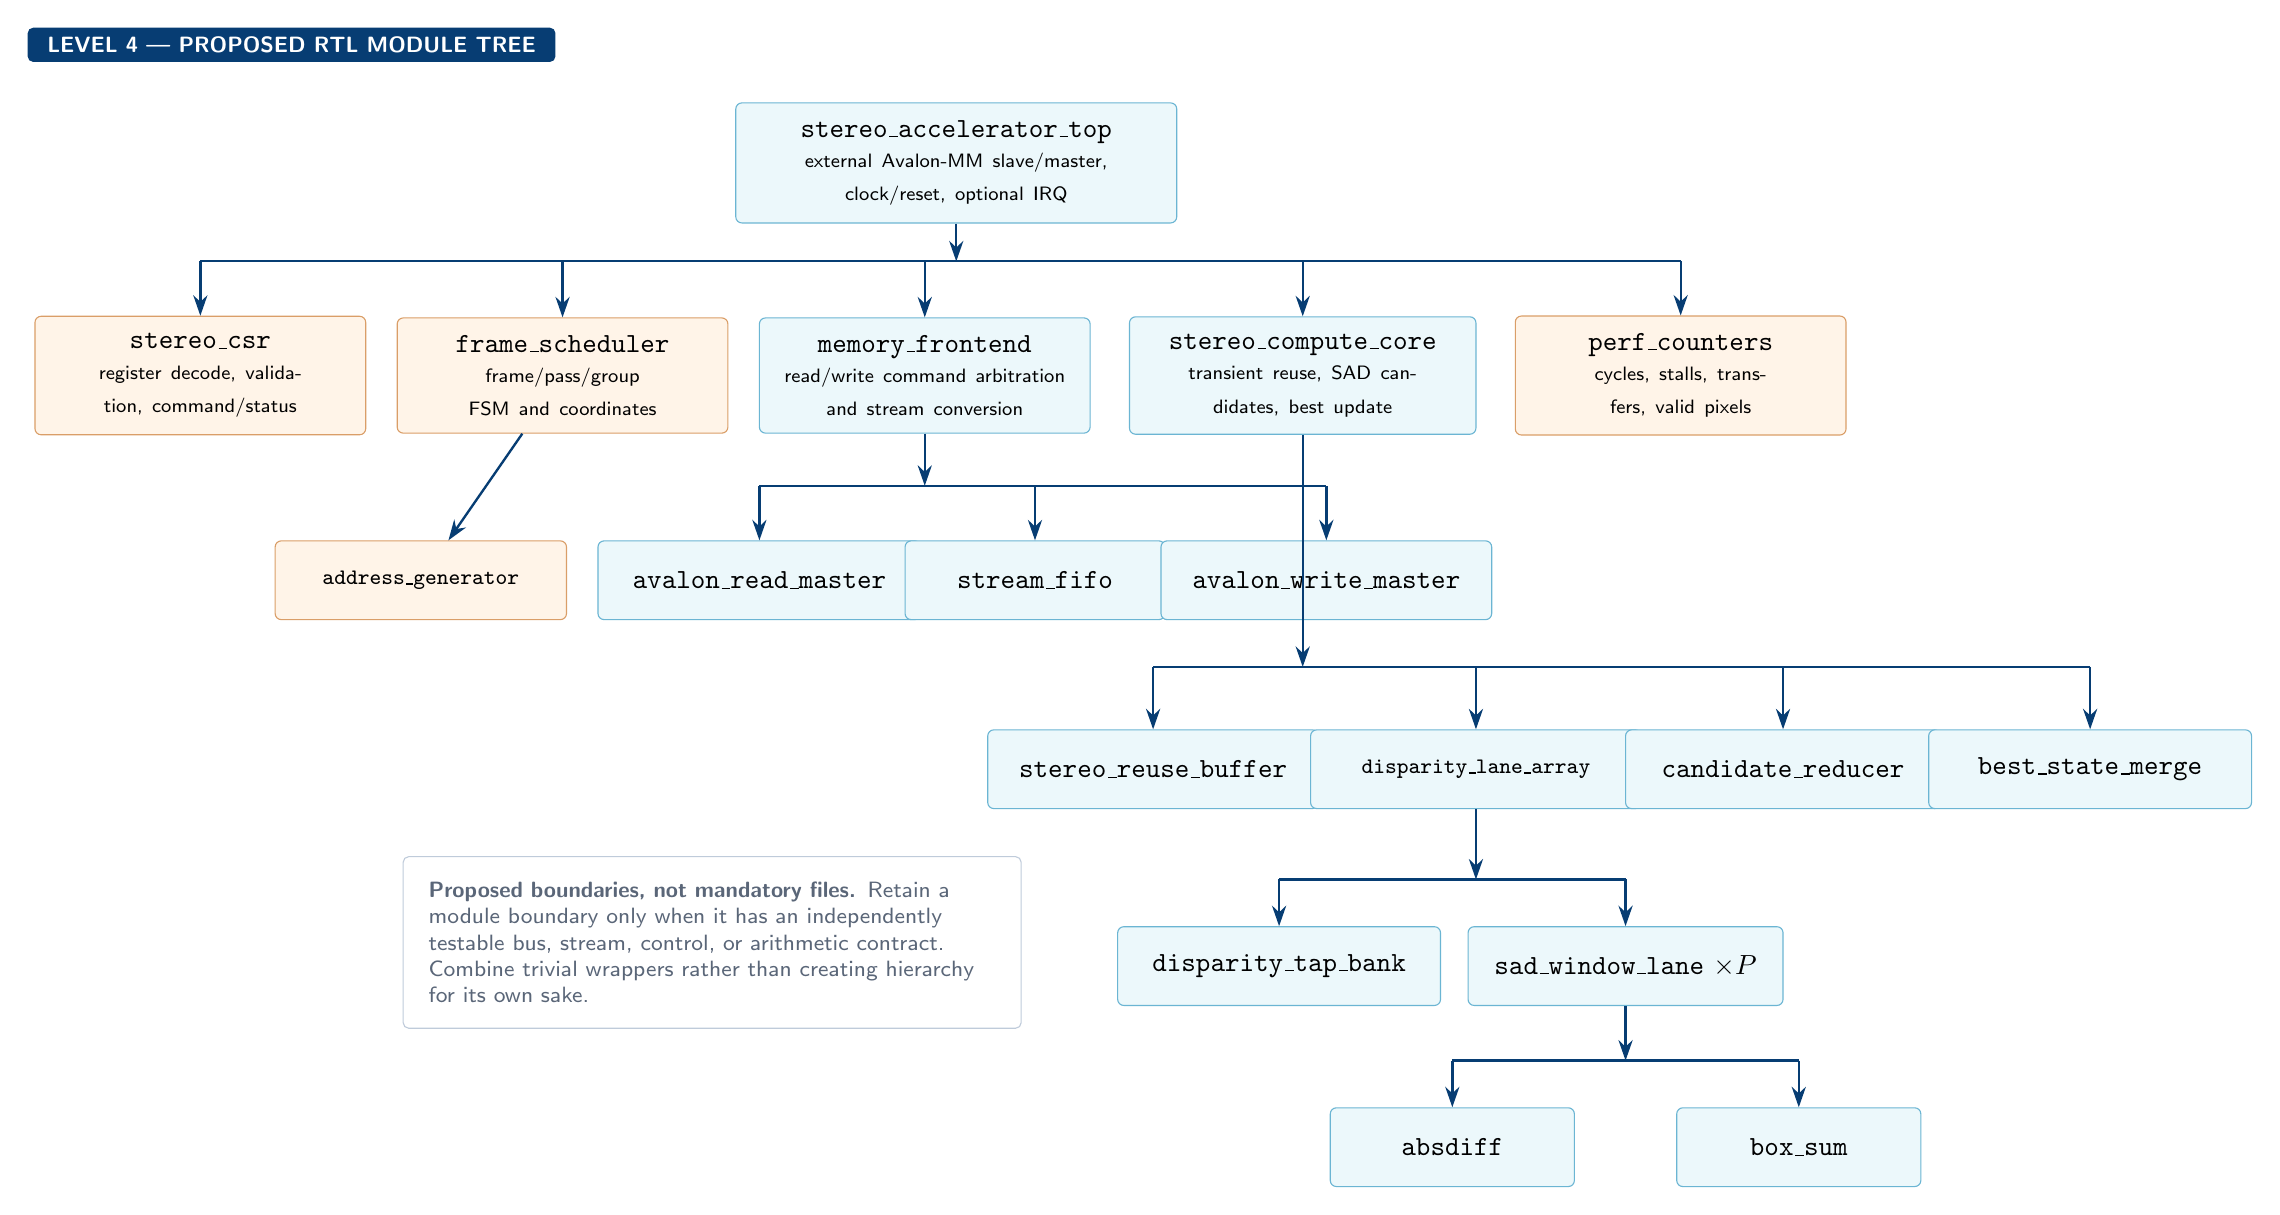
\begin{tikzpicture}[x=1cm,y=1cm]
  \node[labeltag, anchor=west] at (0,0) {LEVEL 4 --- PROPOSED RTL MODULE TREE};
  \node[accel, text width=50mm] (top) at (11.8,-1.5) {\textbf{\texttt{stereo\_accelerator\_top}}\\[-1pt]\scriptsize external Avalon-MM slave/master, clock/reset, optional IRQ};

  \node[control, text width=36mm] (csr) at (2.2,-4.2) {\textbf{\texttt{stereo\_csr}}\\[-1pt]\scriptsize register decode, validation, command/status};
  \node[control, text width=36mm] (scheduler) at (6.8,-4.2) {\textbf{\texttt{frame\_scheduler}}\\[-1pt]\scriptsize frame/pass/group FSM and coordinates};
  \node[accel, text width=36mm] (transport) at (11.4,-4.2) {\textbf{\texttt{memory\_frontend}}\\[-1pt]\scriptsize read/write command arbitration and stream conversion};
  \node[accel, text width=38mm] (core) at (16.2,-4.2) {\textbf{\texttt{stereo\_compute\_core}}\\[-1pt]\scriptsize transient reuse, SAD candidates, best update};
  \node[control, text width=36mm] (perf) at (21.0,-4.2) {\textbf{\texttt{perf\_counters}}\\[-1pt]\scriptsize cycles, stalls, transfers, valid pixels};

  \draw[draw=navy, line width=.8pt] (2.2,-2.75) -- (21.0,-2.75);
  \draw[flow] (top.south) -- (11.8,-2.75);
  \foreach \child in {csr,scheduler,transport,core,perf} {
    \draw[flow] (\child.north |- 0,-2.75) -- (\child.north);
  }

  \node[smallblock, control, text width=31mm, font=\sffamily\footnotesize] (addr) at (5.0,-6.8) {\texttt{address\_generator}};
  \draw[flow] (scheduler) -- (addr);

  \node[smallblock, accel, text width=35mm] (reader) at (9.3,-6.8) {\texttt{avalon\_read\_master}};
  \node[smallblock, accel, text width=27mm] (fifo) at (12.8,-6.8) {\texttt{stream\_fifo}};
  \node[smallblock, accel, text width=36mm] (writer) at (16.5,-6.8) {\texttt{avalon\_write\_master}};
  \draw[draw=navy, line width=.8pt] (9.3,-5.6) -- (16.5,-5.6);
  \draw[flow] (transport.south) -- (11.4,-5.6);
  \foreach \child in {reader,fifo,writer} {
    \draw[flow] (\child.north |- 0,-5.6) -- (\child.north);
  }

  \node[smallblock, accel, text width=36mm] (reuse) at (14.3,-9.2) {\texttt{stereo\_reuse\_buffer}};
  \node[smallblock, accel, text width=36mm, font=\sffamily\footnotesize] (array) at (18.4,-9.2) {\texttt{disparity\_lane\_array}};
  \node[smallblock, accel, text width=34mm] (reduce) at (22.3,-9.2) {\texttt{candidate\_reducer}};
  \node[smallblock, accel, text width=35mm] (merge) at (26.2,-9.2) {\texttt{best\_state\_merge}};
  \draw[draw=navy, line width=.8pt] (14.3,-7.9) -- (26.2,-7.9);
  \draw[flow] (core.south) -- ++(0,-4mm) -| (16.2,-7.9);
  \foreach \child in {reuse,array,reduce,merge} {
    \draw[flow] (\child.north |- 0,-7.9) -- (\child.north);
  }

  \node[smallblock, accel, text width=35mm] (tap) at (15.9,-11.7) {\texttt{disparity\_tap\_bank}};
  \node[smallblock, accel, text width=34mm] (lane) at (20.3,-11.7) {\texttt{sad\_window\_lane} $\times P$};
  \draw[draw=navy, line width=.8pt] (15.9,-10.6) -- (20.3,-10.6);
  \draw[flow] (array.south) -- (18.4,-10.6);
  \draw[flow] (tap.north |- 0,-10.6) -- (tap.north);
  \draw[flow] (lane.north |- 0,-10.6) -- (lane.north);

  \node[smallblock, accel, text width=25mm] (abs) at (18.1,-14.0) {\texttt{absdiff}};
  \node[smallblock, accel, text width=25mm] (box) at (22.5,-14.0) {\texttt{box\_sum}};
  \draw[draw=navy, line width=.8pt] (18.1,-12.9) -- (22.5,-12.9);
  \draw[flow] (lane.south) -- (20.3,-12.9);
  \draw[flow] (abs.north |- 0,-12.9) -- (abs.north);
  \draw[flow] (box.north |- 0,-12.9) -- (box.north);

  \node[note, text width=72mm] (note) at (8.7,-11.4) {\textbf{Proposed boundaries, not mandatory files.} Retain a module boundary only when it has an independently testable bus, stream, control, or arithmetic contract. Combine trivial wrappers rather than creating hierarchy for its own sake.};
  \draw[draw=line, rounded corners=2pt] ([xshift=-2mm,yshift=-2mm]note.south west) rectangle ([xshift=2mm,yshift=2mm]note.north east);
\end{tikzpicture}
\end{document}
